% This is the chapter on sequencing and coverage analysis

\chapter{RNA Sequencing}
\section{Experimental Design}
The primary objective of this research was to provide the first global experimental evidence for both canonical and novel transcripts, their boundaries, and operon structure in \textit{C. acetobutylicum}. For this objective, a strand-specific (ss)RNA sequencing approach was superior to array based and standard RNA-seq approaches for detecting strand-specific signal at high resolution. This technique offers true strand-specific signal, typically with 1-5\% background antisense signal.\cite{18} To identify these transcripts and their features at high resolution and with true strand-specificity, this technique was selected to assess a number of experimental conditions.

A fractional-factorial experimental design was selected to best sample multiple times throughout the \textit{C. acetobutylicum} growth curve (\ref{fig:4.1}) and in response to two fermentation products, butyrate and butanol. This organism responds to resource limitation, acid/solvent stress, and other signals by activating stress response, sporulation, and other stationary-phase systems.\cite{24,37,126} This range of conditions was selected to view transcriptomic responses to growth stage and stress in combination for analysis with ssRNA-seq. 

\begin{figure}[t]
\small
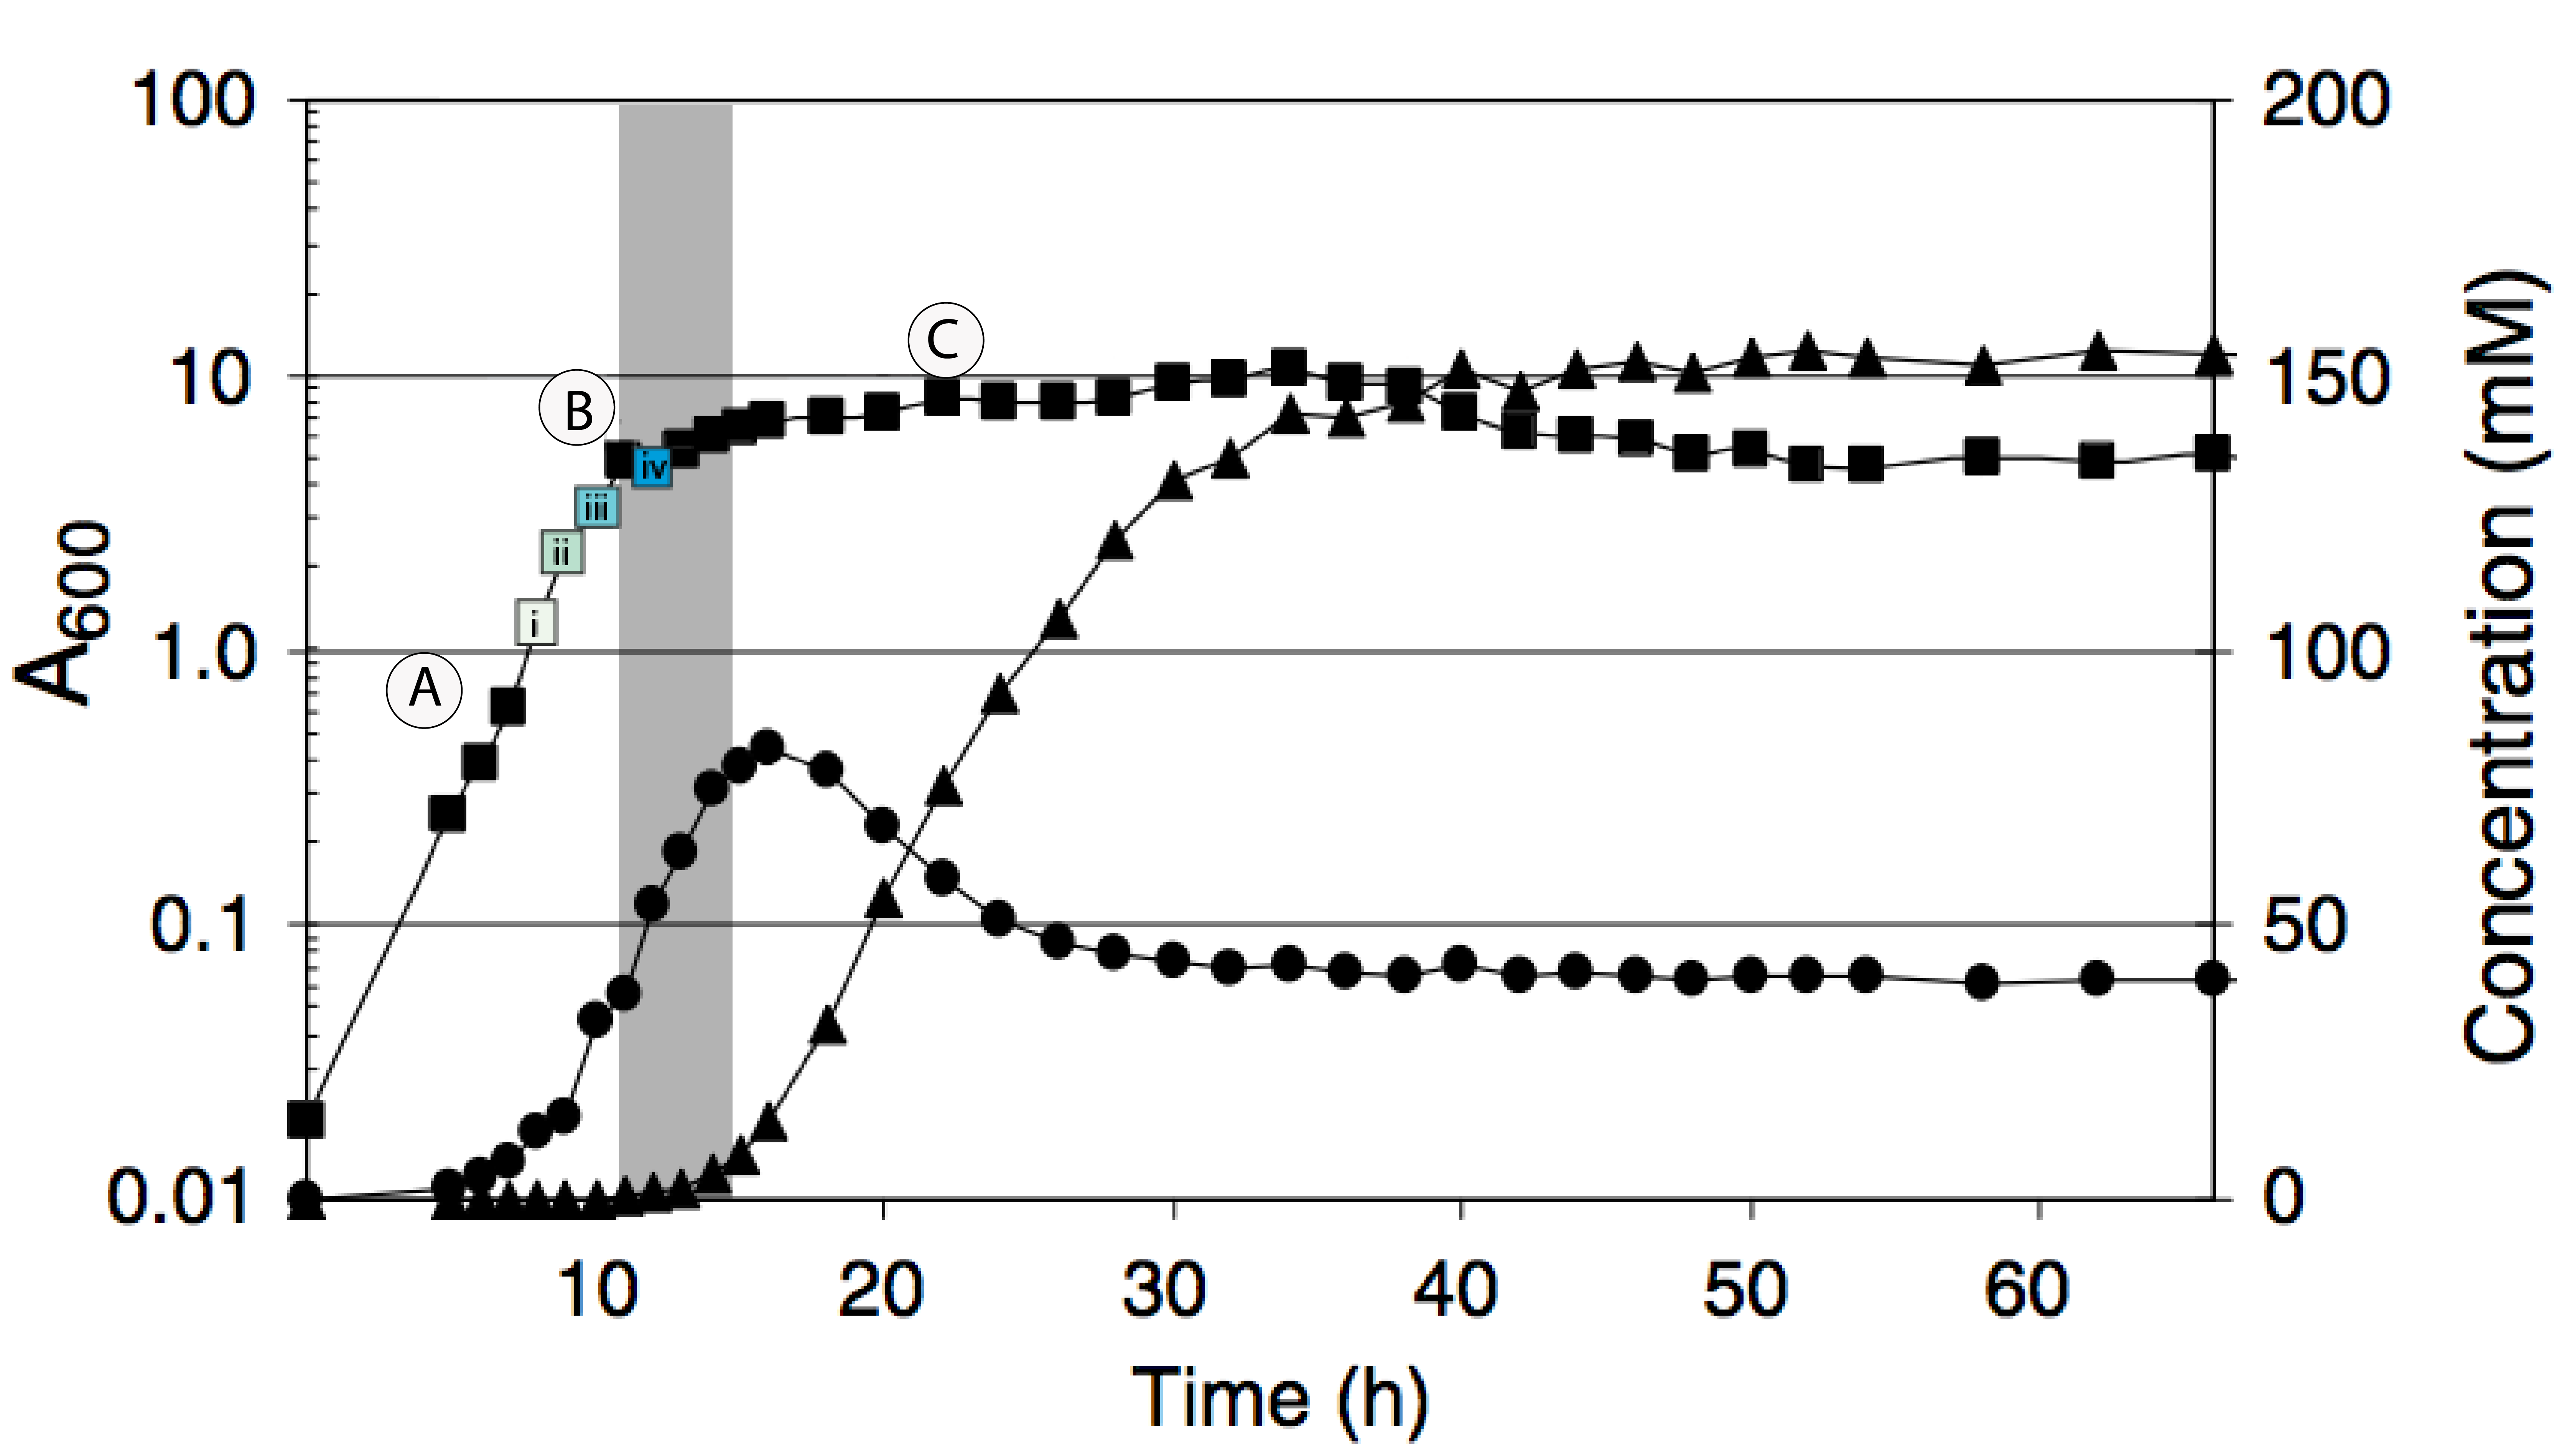
\includegraphics[width=\textwidth,height=3in]{images/Sequencing/Growth_curve.png}
\caption{\textit{C. acetobutylicum} Growth Curve}
\label{fig:4.1}
This growth curve, adapted from Jones \textit{et al.},\cite{180} illustrates the time points selected for the experimental design. After the exponential growth phase (A), \textit{C. acetobutylicum} cells (squares) produce carboxylic acids, such as butyric acid (circles), at increased rates during the transition phase(B). Then, the acids are reassimilated and reduced into solvents such as butanol (triangles) during the stationary phase(C). The stress types butyrate, butanol, and control were assayed in this experiment, in addition to time points 15(i.), 75(ii.), 150(iii.), and 270 minutes (iv.) after synchronization of the cultures at A_{600} of 1.0.
\end{figure}

\section{Desirable Data Qualities}
\subsection{Sequencing Depth}
The success of transcript boundary determination with shotgun-strategy sequencing depends on two signals in the dataset: depth and complexity.\cite{108,109,110,176,177} Here depth of coverage, sequencing depth, or simply depth is defined as the number of reads aligned to a region divided by the size of the region. In the case of a single basepair, this is simply the number of reads overlapping this base. Depth is a useful data quality for identifying absolute differences between fully transcribed and untranscribed regions. Sequencing depth is a complex and over-dispersed random variable\cite{52,53,181} that is non-uniform across a transcript,\cite{179} particularly towards transcript termini.\cite{18} Sequencing depth near transcription start sites has a complicated type II error profile that is a function of sequencing depth due to this bias. This previously discussed(\ref{table:study_compare}) and important signal is frequently used to identify expressed transcripts and their termini.

However, several factors of the experimental procedure affect sequencing depth and are not addressed in most studies. Sequence specific (hexamer,\cite{174} GC\cite{175} bias) or technical issues (background antisense,\cite{18} spurious transcription\cite{164,165}) raise variability and noise of the depth signal and have no existing bioinformatic solution. In contrast, other errors such as DNA contamination, RNA degradation, and overabundant sequences (e.g. rRNA) can be addressed with adjustment to laboratory and analytical workflows. Accounting for these issues during experimental design can improve error rates for reported sequencing depth and depth-based inferences. Specifically, the quantity of useful data in Illumina-based RNA sequencing of prokaryotes can be maximized by acquiring pure, undegraded RNA and removing ribosomal RNA transcripts. Optimal sequencing depth was the first goal for this study to improve error rates and provide a useful sensitivity metric.

\subsection{Library Complexity}
Library complexity is an additional signal that augments the information of sequencing depth. Complexity is the number of unique molecules sequenced by the experiment and can be thought of as the horizontal overlap between aligned reads.\cite{182} Library complexity is desirable for a number of reasons, including decreased loss of sequencing depth to PCR-duplicate reads.\cite{57,182,108} Library complexity can also be translated directly into transcript boundaries using assembly algorithms.\cite{108,58} Algorithmically, the assembly solution's estimates of transcript boundaries improve as both depth and complexity increase. Therefore, high depth and complexity are required for successful assembly of the dataset and determination of transcript boundaries.

Most useful assembly algorithms are overlap consensus or de Bruijn graph based, directly relying on the k-mer complexity of the dataset (where k is an integer and a k-mer is a k-length subsequence of a read) to provide significant overlaps to form the graph.\cite{108,58} Therefore, a large amount of reads (i.e. depth) with long horizontally overlapping segments (i.e. complexity) results in a quality graph that can be traversed by an Eulerian walk. Library complexity results from the fragmentation process and the random sampling of these fragments from the library. However, complexity can be negatively affected by preferential PCR amplification of certain sequences, leading to their over-representation in the final library and dataset.\cite{108,174,175}. Sequencing complexity is a useful data quality for both gene expression and transcriptome mapping studies. A high complexity dataset facilitates transcript boundary identification, especially in the case of low abundance transcripts, and was therefore another goal of this study.

Both depth and complexity are useful data qualities for RNA sequencing studies. Some factors such as sequence specific biases and spurious transcription are largely uncontrollable. However, other intrinsic or technical artifacts can be minimized with minor adjustments to laboratory and analytical workflows, yet they are frequently ignored in the bacterial RNA-seq studies(\ref{table:study_compare}). The poor treatment of these issues in the literature has lead to low and inconsistent coverage, sometimes with ``...less than 60\% genes in the genome had their length completely covered by at least one read''.\cite{115} To avoid regions of zero depth inside of annotated ORFs\cite{115} and false negative errors towards transcript termini, the depth-effecting factors of rRNA-removal, DNA-contamination, and over-amplificiation were optimized. The coverage/complexity signal was used to automate the inference of transcript boundaries and address false positive rates from depth-only inferences. Interestingly, coverage in turn depends on sequencing depth and the fragmentation process, the later of which can be difficult to optimize. In addition to the previously mentioned optimizations, ultra high-depth sequencing(encode ref), with hundreds of millions of non-ribosomal reads, was the appropriate method to improve both coverage and depth for this study. With these data qualities in mind, the following RNA processing workflow was established to produce an ultra high-depth sequencing dataset for transcriptome assembly.



\section{Laboratory Workflow}
A protocol was established to optimize library depth and complexity with hybridization and enzymatic steps(\ref{methods:RNA_prep}). After each RNA manipulation step, the samples were twice washed with 70\% ethanol, stored as precipitates to minimize degradation, and aliquots were taken for quality control. The quality control procedure consisted of spectrophotometric and electrophoretic analyses to ensure RNA purity and integrity. The goals and observations of the quality control process is briefly detailed first.

\subsection{Quality Control}
After washing with ethanol, the absence of salts, divalent cations, and proteins was assessed through spectrophotometry. These contaminants cause RNA degradation or adversely affect the enzymatic reactions of RNA manipulation and library construction. Ratios of absorbance ($\sfrac{\SI{260}{\nano\meter}}{\SI{280}{\nano\meter}}$, $\sfrac{\SI{260}{\nano\meter}}{\SI{230}{\nano\meter}}$) are frequently used to describe the purity of nucleic acid samples, due to purine/pyrimidine absorbance maxima at \SI{260}{\nano\meter}. Observed ratios of 2.0 indicated pure RNA(source), optimal for RNA integrity and library preparation. Afterwards, electrophoretic methods were used to assess ribosomal RNA removal and RNA integrity.

\begin{figure}
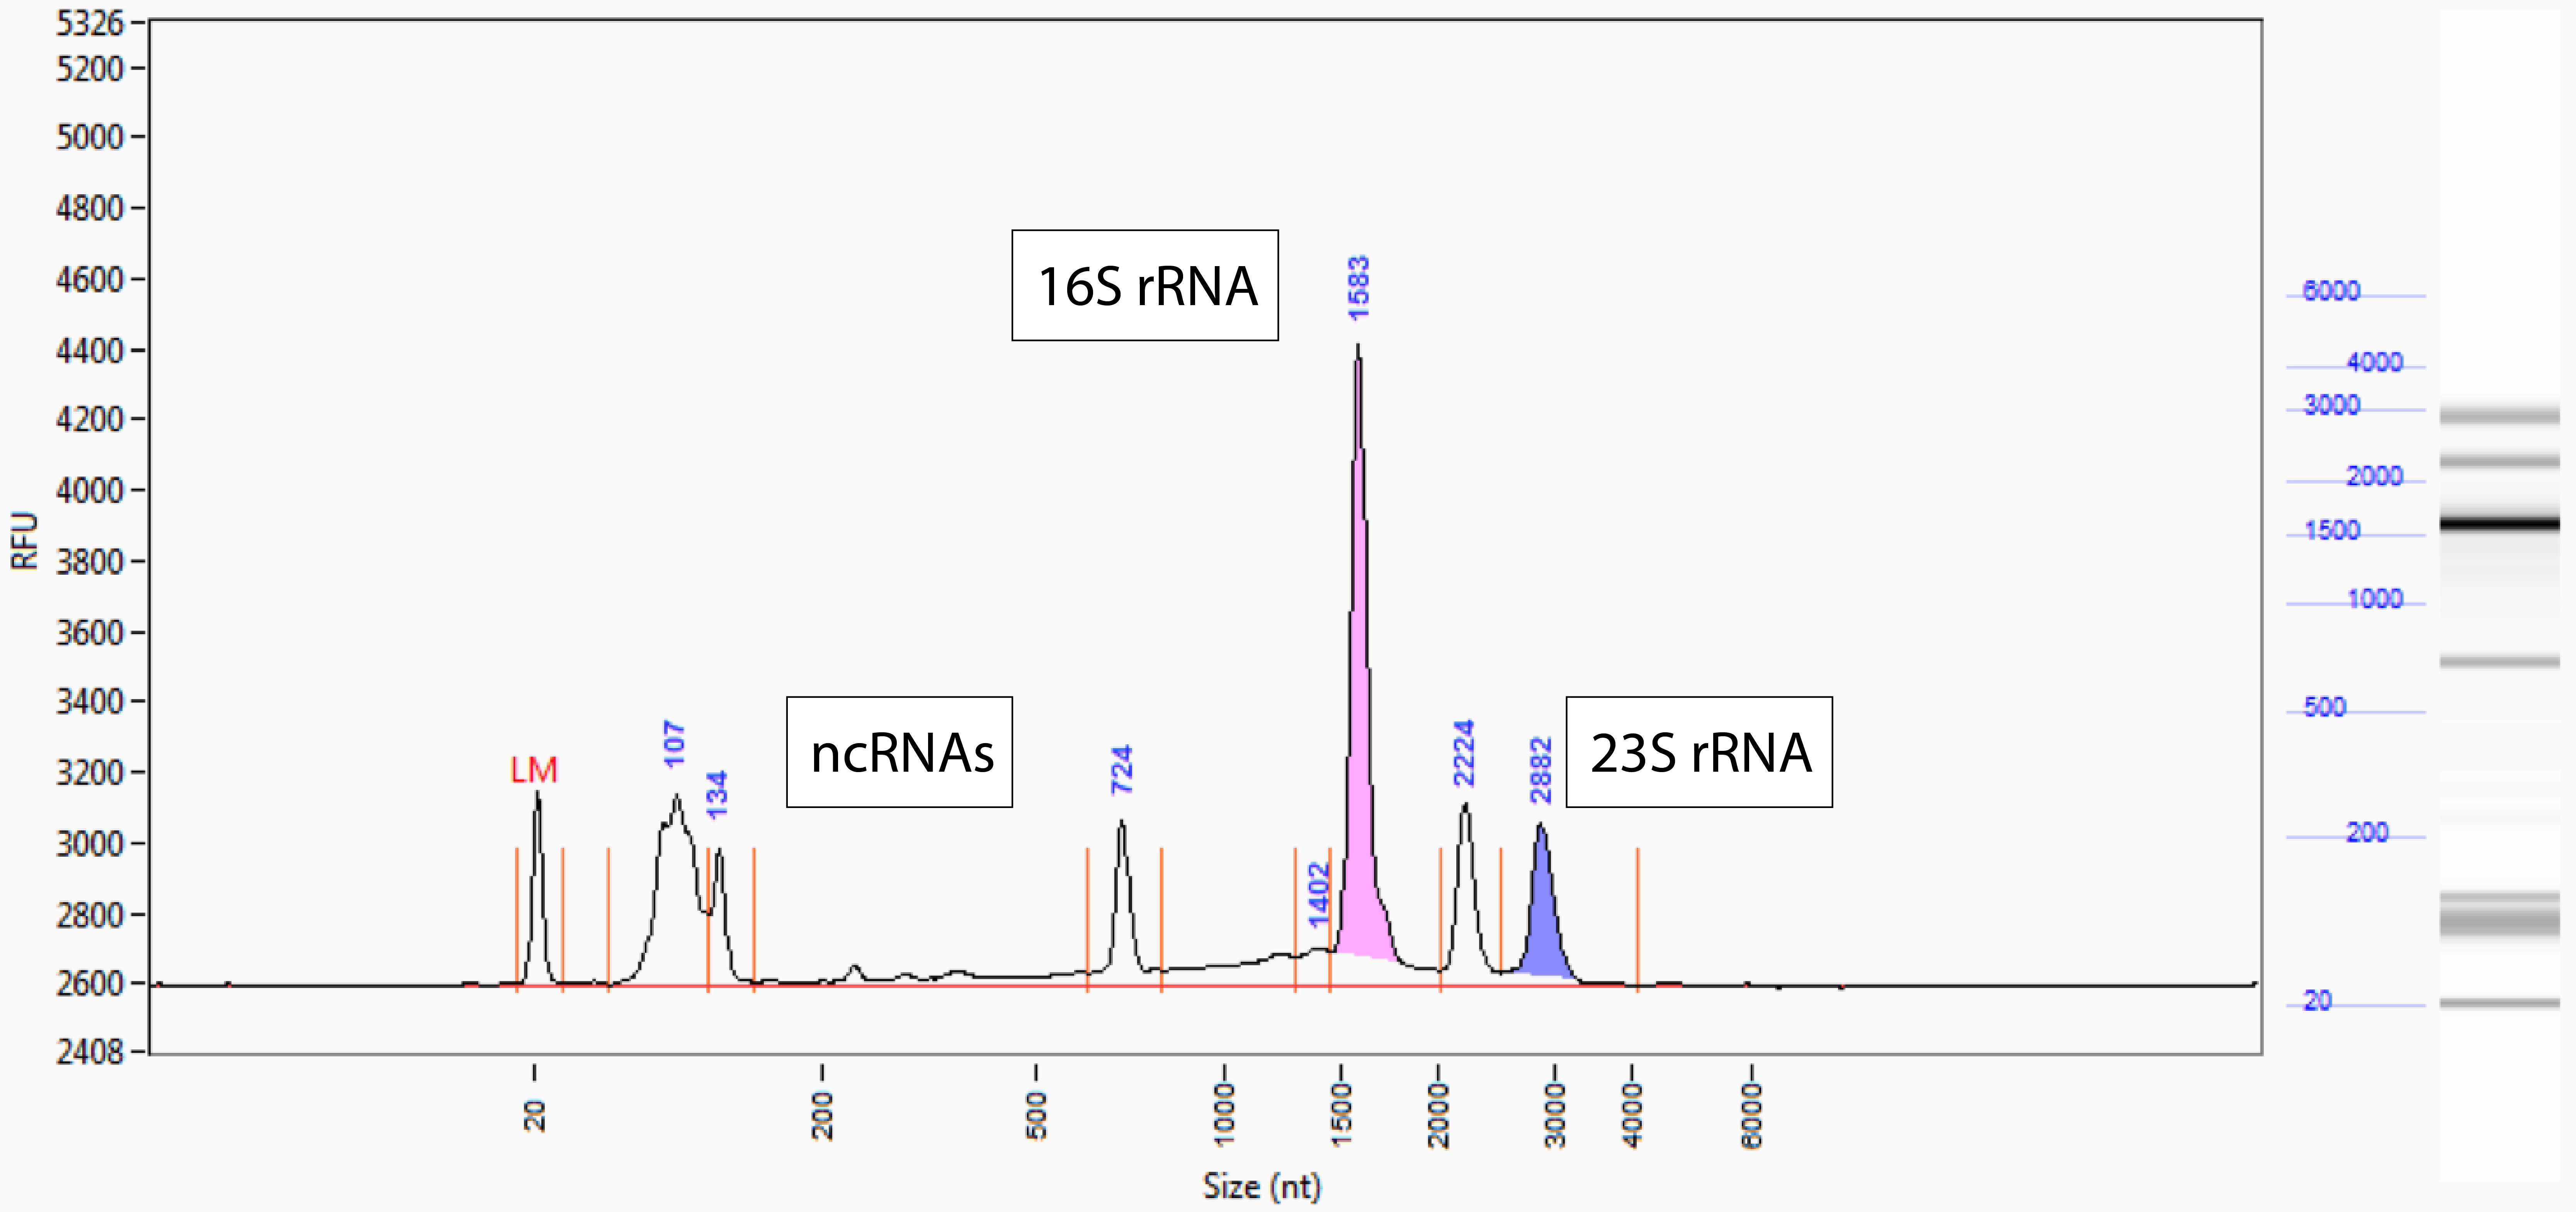
\includegraphics[width=\textwidth,height=3in]{images/Sequencing/RNA-integrity.png}
\caption{RNA Quality}\label{fig:4.2}
In this BioAnalyzer electropherogram, sharp and intact rRNA peaks are visible along with a substantial small RNA population, resulting from the miRNeasy kit used for RNA extraction.
\end{figure}

RNA integrity is commonly analyzed by interpreting ribosomal RNA bands obtained with electrophoretic techniques. Specifically, a small peak width of the rRNA electrophoretic bands with little background signal indicates that the RNA is high quality (e.g. RNA Integrity Number). A representative electropherogram is shown in \ref{fig:4.2}. The results indicate that the RNA was undegraded, with sharp peaks for the 16S and 23S rRNA bands. At each QC step (\ref{fig:4.3}), the RNA had clear pellets, clean spectrophotometric ratios, and the electrophoresis suggested that the RNA were undegraded. The passing samples were then used in subsequent hybridization and enzymatic steps.

\begin{figure}
\hbox to \textwidth{\hfill
\rotatebox{90}{%
\begin{minipage}{\textheight}
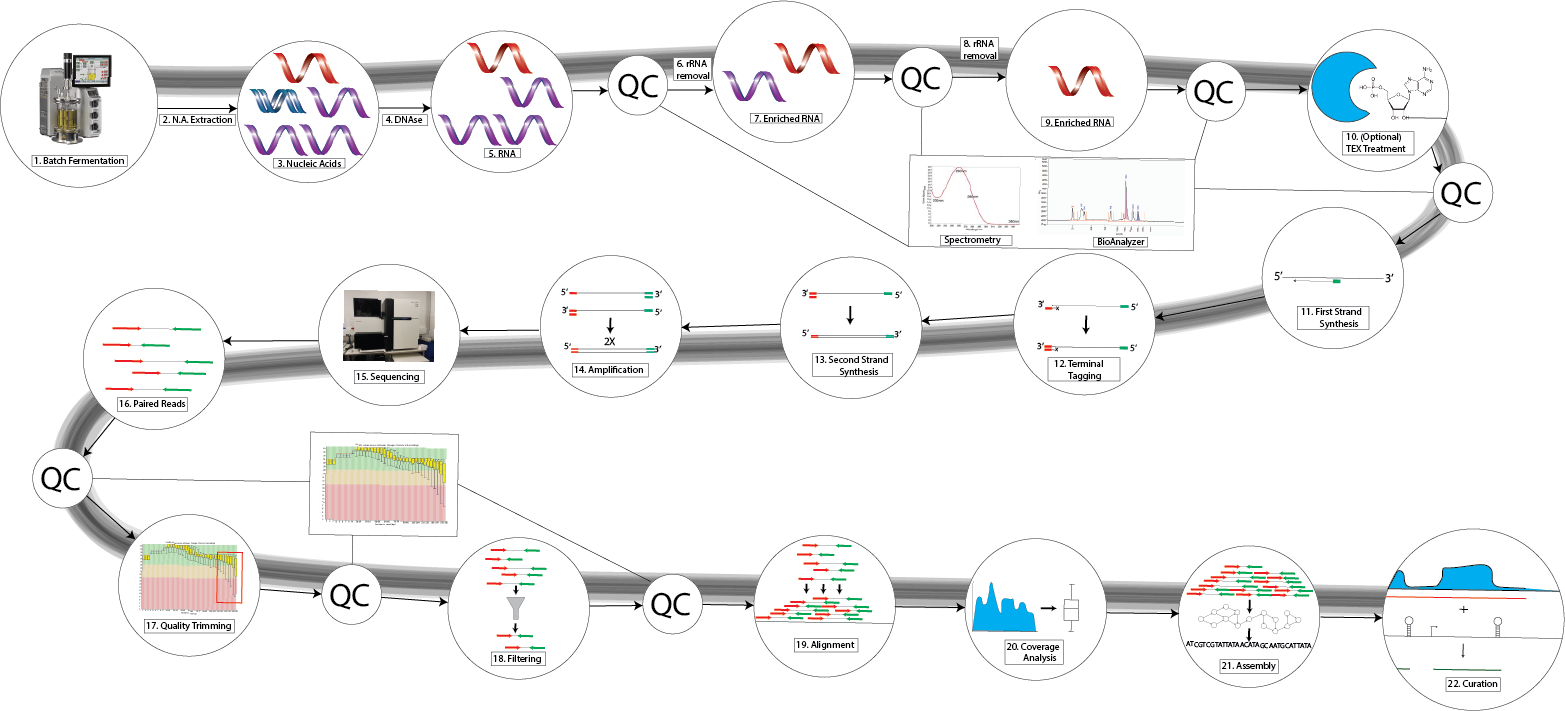
\includegraphics[width=\textheight,height=5in]{images/Sequencing/Workflow.png}
\caption{Laboratory Workflow}\label{fig:4.3}
The laboratory workflow consisted of mRNA enrichment steps and quality control analyses to ensure RNA quality. Ligation-free library preparation resulted in paired-end Illumina reads for preprocessing, alignment, analysis, and assembly.
\end{minipage}}\hfill}
\end{figure}


\subsection{mRNA/sRNA Enrichment}
The previous subsection discussed quality control measures that were used for initial and stepwise assessment of RNA samples. To produce a high quality sequencing dataset, RNA manipulations enriched primary transcripts (mRNAs and sRNAs) and minimized background signal (e.g. degraded transcripts, DNA) through RNA manipulations(\ref{fig:4.3}). After extraction, residual DNA was removed with DNAse treatment (Step 4., \ref{fig:4.3}). After verifying the initial total RNA samples with the QC procedure, ribosomal RNA(rRNA) was removed with the MicrobExpress hybridization method. After additional QC, the primary transcripts were further enriched with an additional round of rRNA removal. Then selected samples - technical replicates of 2 times points(75 and 270 minutes) and all stress types (6 total) - were treated with a 5'-phosphate specific exonuclease (TEX), enriching for primary transcripts further. Primary transcripts such as mRNAs and sRNAs are produced with a 5'-NTP. Post-transcriptional processing of primary transcripts (e.g. endonucleolytic cleavage) results in 5'-monophosphate ends, which are preferred by the TEX exonuclease. The TEX treatment thus removed rRNA and degraded transcripts in these samples. This workflow maximized depth and complexity in the results by removing DNA, rRNA, and degraded transcripts. After a final QC checkpoint the enriched samples were used for library preparation(\ref{fig:4.3}) and sequencing.


\section{Data Processing, Alignment, and Coverage Analysis}
The libraries were sequenced paired-end over 5 lanes of an Illumina HiSeq 2500, producing 1.5 billion 76bp reads, averaging ~25 million clusters/pairs per library(App. \ref{app:read_summary}). The reads were then processed through a customized bioinformatic workflow (\ref{methods:data_proc_aln}). K-mer content, read length, GC-content, and additional basic qualities were assessed to ensure the quality of the unprocessed reads. Next, low-quality bases were removed to raise the quality of the sequenced bases to acceptable levels(\ref{methods:read_process_align}). Then, sequence reads from remaining ribosomal RNAs were removed \textit{in silico}. After two rounds of hybridization-based removal, signal from ribosomal RNA was reduced from 95\%(bacterial rRNA removal source) to 62\%, representing a 7.6-fold enrichment of primary transcripts. Finally, 97\% of the reads aligned to the \textit{C. acetobutylicum} genome (\ref{fig:4.3}). Of these, 7.75M(83\%) reads per sample were properly paired, that is, both mates of each pair were in the correct orientation. In total, 458,814,860 perfectly-paired non-ribosomal reads were produced and then used for subsequent analysis.

\begin{figure}
\small
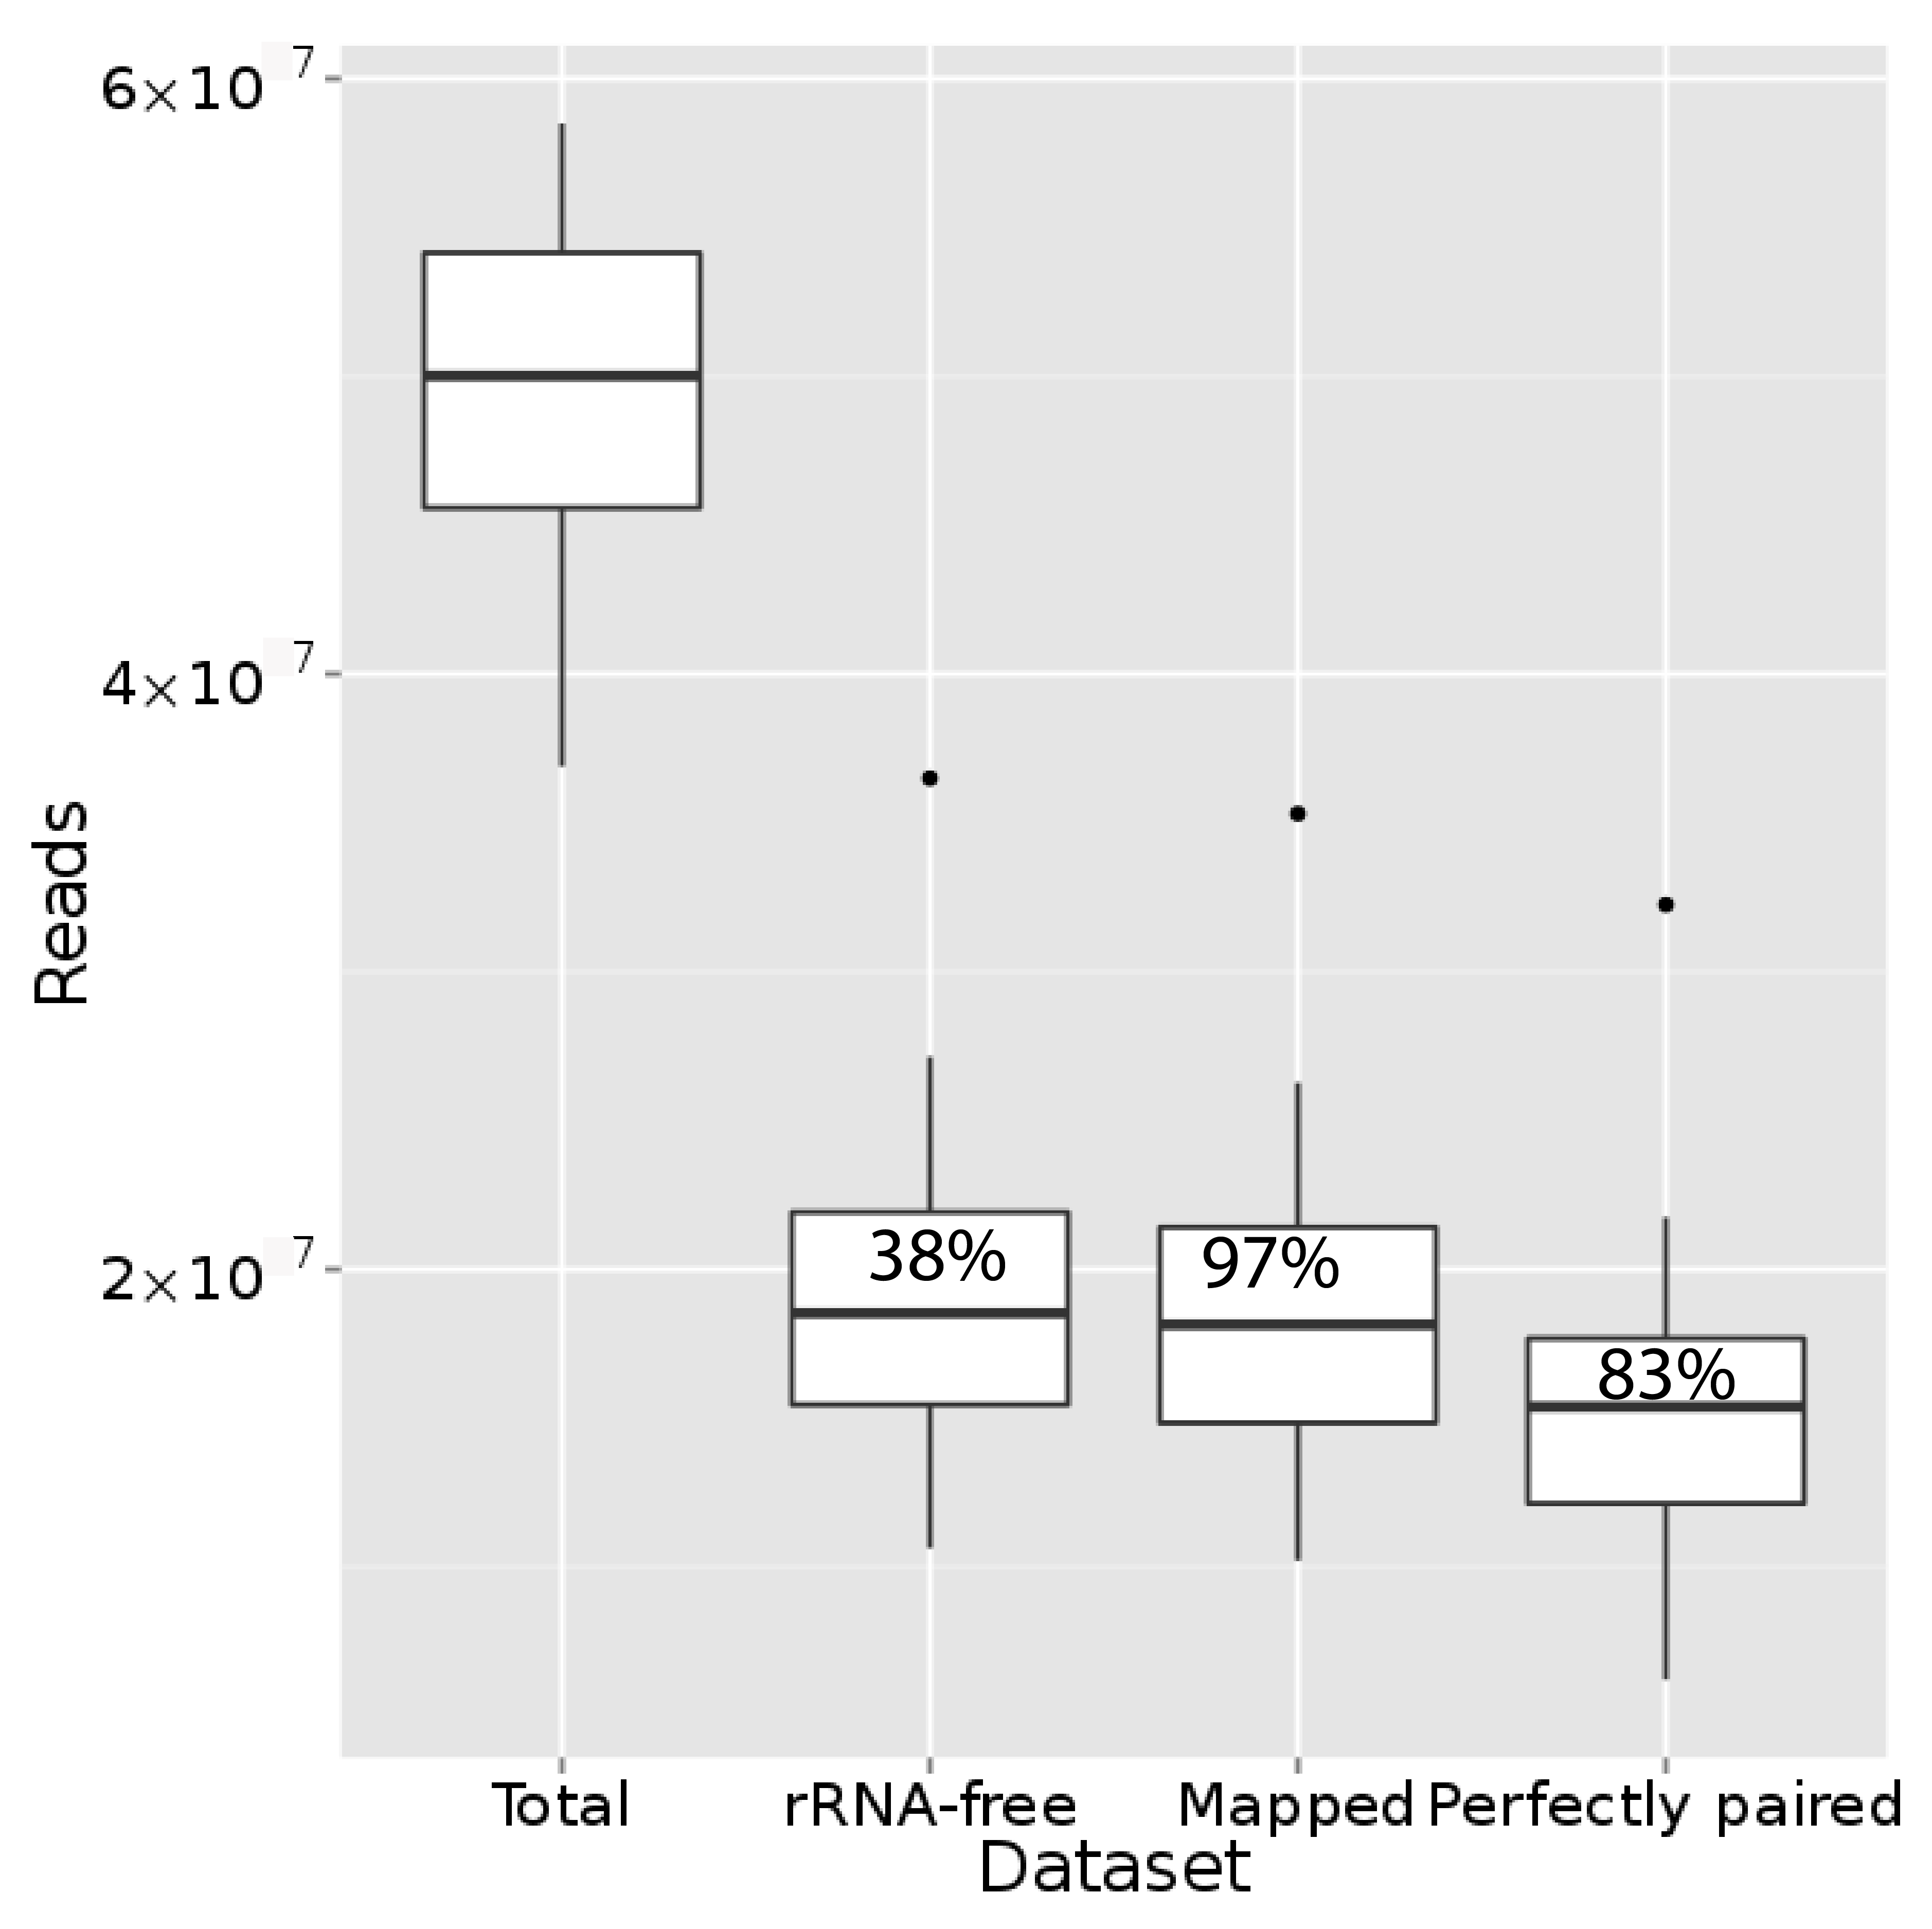
\includegraphics[width=\textwidth,height=5in]{images/Sequencing/Alignment_reads.png}
\caption{Sequence Read Processing and Alignment}\label{fig:4.4}
An average of 50 million reads (25M clusters/pairs; left) was produced for each of the 30 libraries. Ribosomal RNA reads were then filtered and the remaining reads (middle left) were then aligned to the genome (middle right). Of these, 83\% were properly paired reads (right), ideal for transcriptome assembly.
\end{figure}

However, the number of reads alone are a poor indicator of the sensitivity of an experiment; the distribution of these data throughout the genome is preferable, but is infrequent in similar studies(\ref{table:study_compare}). To better understand the depth of sequencing, it was desirable to determine the per-base sequencing depth throughout the genome. Two methods are frequently used to quantify and summarize depth. The first approach is referred to as ``fold-coverage,'' calculated by summing the number of sequenced bases divided by the estimated size of the transcriptome or genome. However, the underlying assumption of a uniform distribution of reads is not valid for transcriptomic sequencing. A more precise approach is the second approach, calculating sequencing depth directly. By summing the number of reads aligned to each base, central tendency measures of the resulting distribution are precise estimates of per-base sequencing depth across the genome. No single average sequencing depth is more significant than another (e.g. 10x vs 9x), although increasing depth provides additional terminal reads for transcript boundary identification. 

Empirically, it seems that a coverage of 100-200 million(M) 100bp paired-end reads is sufficient to detect low abundance transcripts in the 60-140 megabase(Mb) hg19 human transcriptome,\cite{110} although other studies claim that this number could be as high as 700M.\cite{185} This sums to 20-40 gigabases(Gb) of sequencing, 120-660 times the conservative estimate of the size of the human transcriptome. In the case of \textit{C. acetobutylicum}, the maximum possible size of the transcriptome is 8.2Mb, with a realistic estimate of 4-6Mb. With the 450M properly-paired reads described here, 68.7 Gb were sequenced for a much smaller transcriptome, approximately 11-17 thousand times its length. This estimate suggests that, cumulatively, this study achieves comparable or superior fold-coverage than recommended by these guidelines using the first method for depth calculation. 

In terms of actual sequencing depth, however, requirements for bacterial transcriptome sequencing are unknown despite recent efforts\cite{108,109,110,176,177} and differing views on detection limits.\cite{176,186} In this study, the definition of ideal ``coverage'' is strictly a sequencing depth greater than one from one transcript boundary to another. In most species, these boundaries are unknown and their identification is complicated by uneven sequencing depth at transcript termini.\cite{18} The discovery of transcript start and stop sites thus depends on per-base sequencing depth computed using the second method above.
\begin{figure}
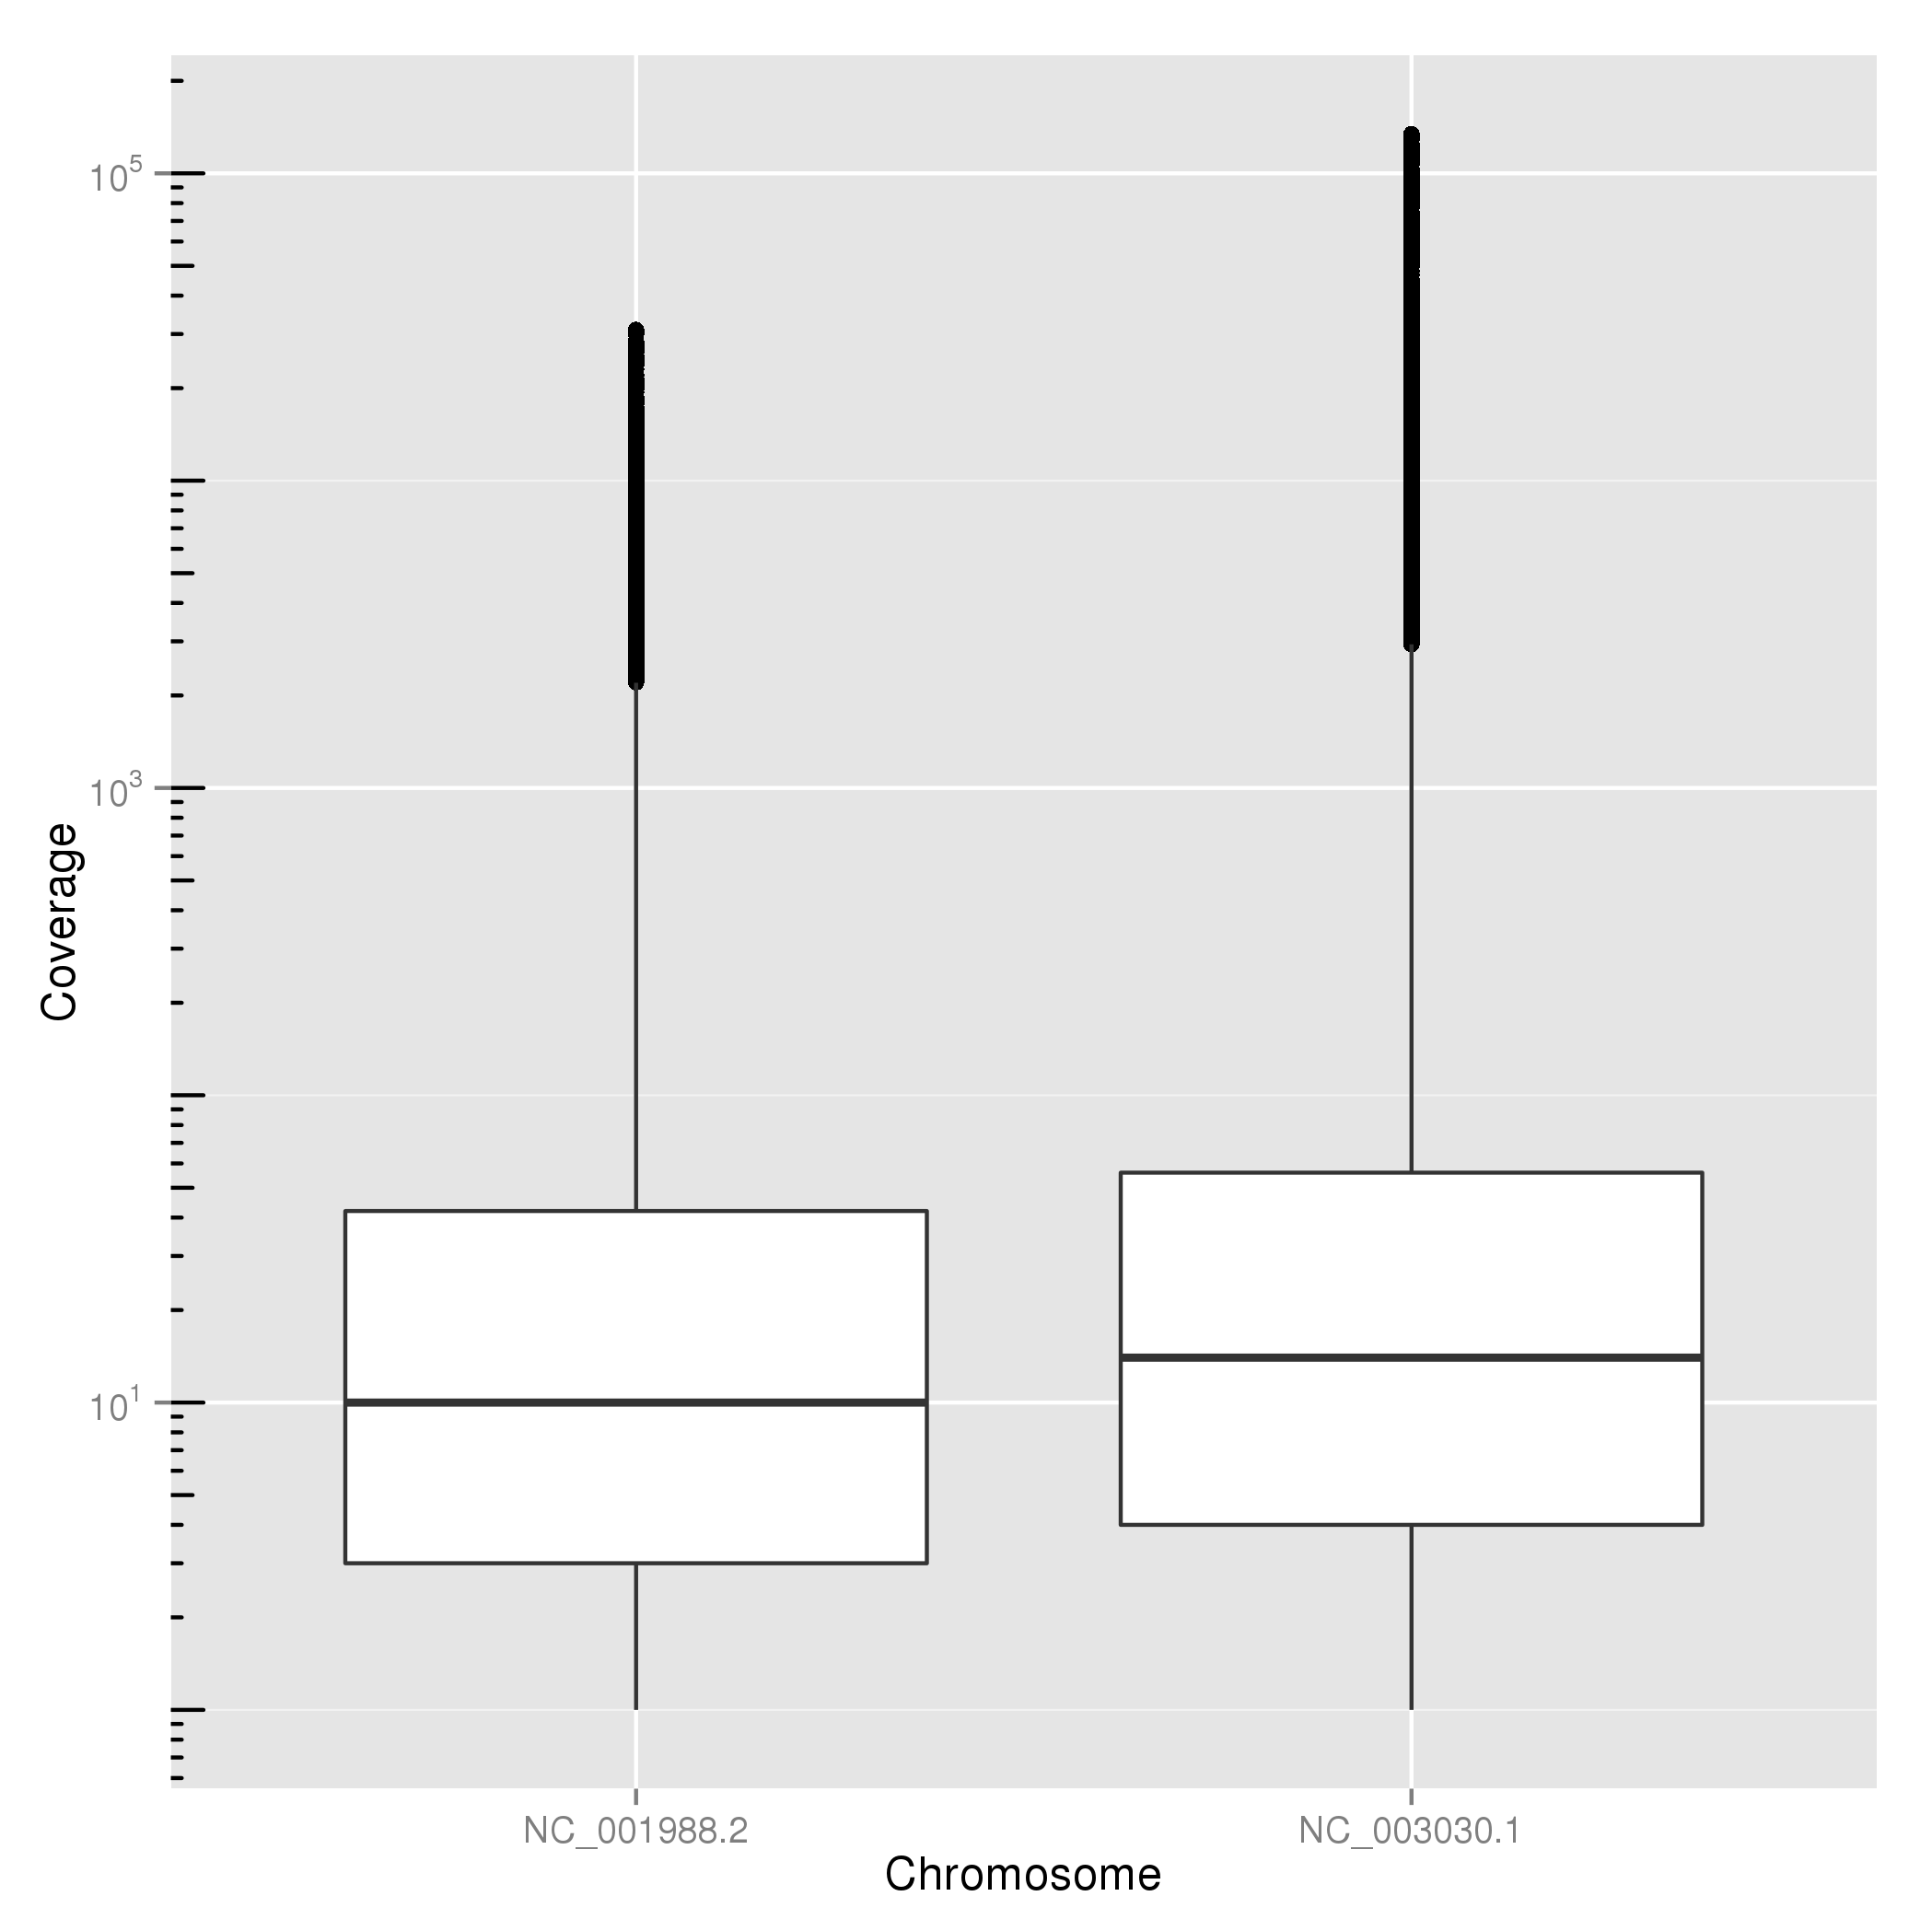
\includegraphics[width=\textwidth]{images/Sequencing/Supplemental/BA-A-75+boxplot.png}
\caption{Representative Per-base Sequencing Depth}\label{fig:4.5}
These boxplots show the distribution of per-base sequencing depth throughout the pSOL1 megaplasmid (left) and the \textit{C. acetobutylicum} chromosome (right) for a single library. The median depth in each library was greater than 10x.
\end{figure}

A median of > 10x coverage per base and per strand was observed for each of the 30 libraries (\ref{fig:4.5}). Cumulatively, the median per base coverage is 156x throughout the genome(\ref{fig:4.6}), generally considered very deep. The median depth in truly transcribed regions is greater as shown in the next chapter. To clarify, some of the depth described by this distribution(\ref{fig:4.6}) was due to previously discussed background signals such as DNA contamination\cite{176} or spurious transcription.\cite{164,165} Background signal is indeed a pressing concern for RNA-seq,\cite{110,176,57} complicating the determination of transcript boundaries. After describing read counts, fold-coverage, and per-base sequencing depth it is clear that this study possesses unprecedented sensitvity for transcriptome mapping.

\begin{wrapfigure}{l}{0.4\textwidth}
\small
\vspace{-20pt}
\begin{center}
{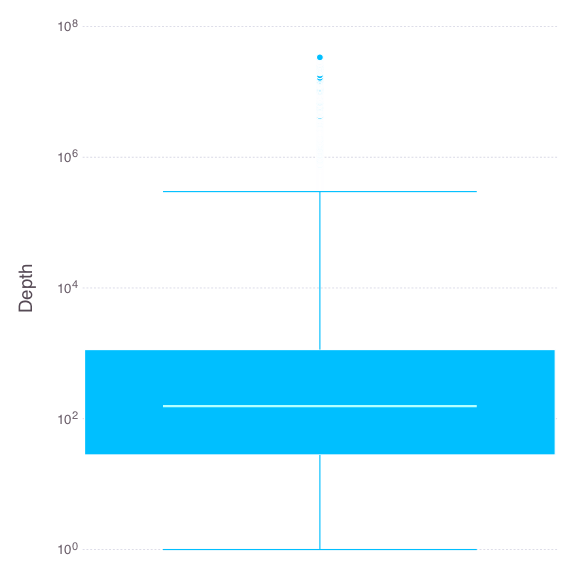
\includegraphics[width=\linewidth,height=3in]{images/Sequencing/Cumulative_depth_boxplot.png}}
\caption{Cumulative Depth Boxplot}\label{fig:4.6}
The distribution of per-base sequencing depth illustrates high sensitivity.
\end{center}
\vspace{-20pt}
\end{wrapfigure}


In summary, the data suggested a successful first aim for this project: a quality RNA-seq dataset for subsequent assembly and annotation. The experiment and RNA processing protocol were designed with depth and complexity in mind. Primary transcripts were enriched and contaminants were removed, controlling for RNA purity and integrity after each manipulation. Thirty samples were sequenced over six lanes, resulting in 1.5 billion reads, with 458 million properly-paired reads aligning to the genome. Analysis of the aligned sequences demonstrated consistently high primary transcript enrichment, alignment rates, and sequencing depth. This depth of signal is comparable or superior to many similar studies in prokaryotes and to guidelines for human genome sequencing.



